% written by Akmal Zuhdy Prasetya (H071191035)

\documentclass[peerreview]{IEEEtran}
\usepackage{cite} % Tidies up citation numbers.
\usepackage{url} % Provides better formatting of URLs.
\usepackage[utf8]{inputenc} % Allows Turkish characters.
\usepackage{amsmath}
\usepackage{booktabs} % Allows the use of \toprule, \midrule and \bottomrule in tables for horizontal lines
\usepackage{graphicx}
\usepackage{float}
\usepackage{adjustbox}
\usepackage{hyperref}
\hypersetup{
    colorlinks=true,
    linkcolor=black,
    filecolor=magenta,      
    urlcolor=cyan,
    citecolor=black,
    pdfpagemode=FullScreen,
    }

\urlstyle{same}
\usepackage[justification=centering]{caption}

\hyphenation{op-tical net-works semi-conduc-tor} % Corrects some bad hyphenation

\graphicspath{{images/}}

\begin{document}
%\begin{titlepage}
% paper title
% can use linebreaks \\ within to get better formatting as desired
\title{CycleGAN Model Implementation Report Using Tensorflow - UNHAS Final Test Project}


% author names and affiliations

\author{Akmal Zuhdy Prasetya \\
Information Systems Study Program \\
Department of Mathematics \\
Hasanuddin University\\
}
\date{6/17/22}

% make the title area
\maketitle
\tableofcontents
\listoffigures
\listoftables
%\end{titlepage}

\IEEEpeerreviewmaketitle
\begin{abstract}
Image-to-image translation is an important topic in the field of computer vision. It aims to learn the mapping between input image and output image by training the datasets, and finally translates the image style from one domain to another. In terms of the form of translation, it can be divided into the translation between two domains and multiple domains from different datasets. And it is also divided into pairs and unpaired by the training datasets. As a successful representation of the translation of an unpaired image between two domains, the CycleGAN model is of great significance to the research and application. Starting from the application background of the CycleGAN model, this paper attempts to show an implementation of CycleGAN using Tensorflow to try transforming some images into another style so we can better understand how CycleGAN works.

\end{abstract}


% INTRODUCTION
\section{Introduction}

Since the arrival of Convolutional Neural network (CNN), deep learning as an implementation algorithm of machine learning, has been widely used in Computer Vision field, from the beginning of the recognition of handwritten, object tracking, speech recognition, face recognition, and through training of fruit images dataset, help person determine the type of fruit when given image about it, until Alpha Go, it is the first computer program to defeat a professional human Go player, the first program to defeat a Go world champion, and arguably the strongest Go player in history, making the deep reinforcement learning attracted more and more researcher's attention.

At the same time, the famous model GAN (Generative Adversarial Networks) proposed by Goodfellow in 2014 \cite{goodfellow2014generative}, which is considered to be the coolest idea in the field of machine learning in the past 20 years and bring new breakthroughs to the deep learning model. The key to GAN's success is the idea of an adversarial loss that forces the generated images to be, in principle, indistinguishable from real photos. This loss is particularly powerful for image generation tasks, as this is exactly the objective that many of computer graphics aims to optimize \cite{zhu2019brief}.


% PROBLEM DEFINITION
\section{Problem Definition}
In this technical report, I focus on reproducing an implementation of CycleGAN model to translate or transform a some images into another style using Tensorflow to better understand how CycleGAN works.


% MODEL EXPLANATION
\section{CycleGAN Architecture}
In this section, we first briefly review the principle of CycleGAN and then give a comparison with the Pix2Pix GAN model image-to-image translation models.

\subsection{Background of CycleGAN}
The task of image style translation is to change a particular aspect of a given image to another, that is to say, given any two unordered image collections X and Y, the algorithm learns to automatically “translate” an image from one into the other and vice versa, which can be divided into two situations which is one is paired translation and the other is unpaired translation \cite{upadhyay2021uncertainty}.

\begin{figure}[H]
    \centering
    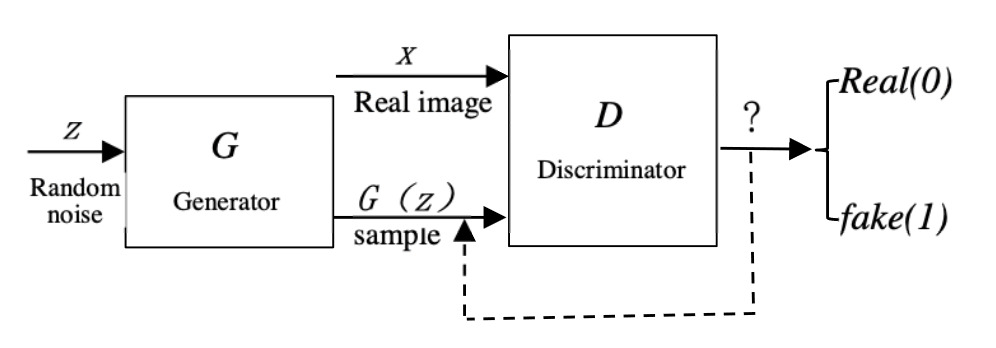
\includegraphics[width=0.8\columnwidth]{GAN Model}
    \caption{GAN Model}
    \label{fig:s=gan_model}
\end{figure}

For image translation in pairs, the commonly used models is Pix2Pix \cite{isola2017image}, it can verify by example that pix2pix model has a certain universality, but also has certain limitation. First of all, the requirements of the training dataset of training samples must be in pairs, but in real life, if you want to collect a large number of data in pairs, it is a little difficulty. If the data quantity is little, and there will be a fitting, model training effect. Secondly, the image transfer achieved by this model is only limited to the transformation of different styles of the same image, such as color changes. At this time, how to use samples with different styles for training to complete the translation of image style is the basic design idea of CycleGAN model.

\subsection{CycleGAN Model Review}
As one of the most interesting and important deep learning achievements in 2017, CycleGAN has many application in the past two years. The original schematic and formula of the CycleGAN paper are as follows.

\begin{figure}[H]
    \centering
    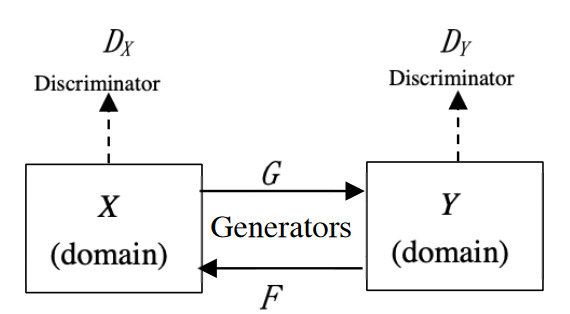
\includegraphics[width=0.8\columnwidth]{CycleGAN Model}
    \caption{CycleGAN Model}
    \label{fig:s=cyclegan_model}
\end{figure}

Jun-Yan Zhun \cite{zhu2017unpaired} given two datasets $\{x_i\}(i=1$ to $M)$ and $\{y\}(j=1$ to $N)$, collected from two different domains $X$ and $Y$, where $x_i \in X$ and $y_j \in Y$, the goal of CycleGAN is to learn a mapping function: $G:X \to Y$, such that the distribution of images from $G(X)$ is distinguishable from the distribution $Y$ using adversarial loss.

CycleGAN contains two mapping functions $G:X \to Y$ and $F:Y \to X$. Two adverasial discriminators $D_X$ and $D_Y$ are proposed to distinguish whether images are translated from another domain. CycleGan applies the GAN framework to train the generative and discriminative models jointly. The overall CycelGAN loss function is expressed as follows: 

\begin{equation}
    \begin{split}
         V(G, F, D_X, D_Y) & = V_GAN(D_Y, G, X, Y) \\
         & + V_GAN(D_X, F, Y, X) \\
         & + \lambda V_cyc(G, F)
    \end{split}
\end{equation}

Where $V_GAN(D_Y, G, X, Y)$ and $V_GAN(D_X, F, Y, X)$ are the loss function for mapping functions $G$ and $F$, and for the discriminators $D_Y$ and $D_X$ is the cycle consistency loss that forces $F(G(x)) \approx x$ and $G(F(y)) \approx y$, in which each image can be reconstructed after a cycle mapping. \lambda penalizes the importance between $V_GAN$ and $V_cyc$.


% ANALYSIS / IMPLEMENTATION
\section{CycleGAN Implementation}
In general, it can be seen that ...


% CONCLUSION
\section{Results and Conclusions}
Based on the results obtained, CycleGAN is

% references
\bibliographystyle{plain} % We choose the "plain" reference style
\bibliography{refs} % Entries are in the refs.bib file

\end{document}


